%%%%%%%%%%%%%%%%%%%%%%%%%%%%%%%%%%%%%%%%%
% Journal Article
% LaTeX Template
% Version 1.3 (9/9/13)
%
% This template has been downloaded from:
% http://www.LaTeXTemplates.com
%
% Original author:
% Frits Wenneker (http://www.howtotex.com)
%
% License:
% CC BY-NC-SA 3.0 (http://creativecommons.org/licenses/by-nc-sa/3.0/)
%
%%%%%%%%%%%%%%%%%%%%%%%%%%%%%%%%%%%%%%%%%

%----------------------------------------------------------------------------------------
%	PACKAGES AND OTHER DOCUMENT CONFIGURATIONS
%----------------------------------------------------------------------------------------

\documentclass[twoside]{article}

\usepackage{lipsum} % Package to generate dummy text throughout this template

\usepackage[sc]{mathpazo} % Use the Palatino font
\usepackage[T1]{fontenc} % Use 8-bit encoding that has 256 glyphs
\linespread{1.05} % Line spacing - Palatino needs more space between lines
\usepackage{microtype} % Slightly tweak font spacing for aesthetics

\usepackage[hmarginratio=1:1,top=32mm,columnsep=20pt]{geometry} % Document margins
\usepackage{multicol} % Used for the two-column layout of the document
\usepackage[hang, small,labelfont=bf,up,textfont=it,up]{caption} % Custom captions under/above floats in tables or figures
\usepackage{booktabs} % Horizontal rules in tables
\usepackage{float} % Required for tables and figures in the multi-column environment - they need to be placed in specific locations with the [H] (e.g. \begin{table}[H])
\usepackage{hyperref} % For hyperlinks in the PDF

\usepackage{lettrine} % The lettrine is the first enlarged letter at the beginning of the text
\usepackage{paralist} % Used for the compactitem environment which makes bullet points with less space between them

\usepackage{abstract} % Allows abstract customization
\renewcommand{\abstractnamefont}{\normalfont\bfseries} % Set the "Abstract" text to bold
\renewcommand{\abstracttextfont}{\normalfont\small\itshape} % Set the abstract itself to small italic text

\usepackage{titlesec} % Allows customization of titles
\renewcommand\thesection{\Roman{section}} % Roman numerals for the sections
\renewcommand\thesubsection{\Roman{subsection}} % Roman numerals for subsections
\titleformat{\section}[block]{\large\scshape\centering}{\thesection.}{1em}{} % Change the look of the section titles
\titleformat{\subsection}[block]{\large}{\thesubsection.}{1em}{} % Change the look of the section titles

\usepackage{fancyhdr} % Headers and footers
\pagestyle{fancy} % All pages have headers and footers
\fancyhead{} % Blank out the default header
\fancyfoot{} % Blank out the default footer
\fancyhead[C]{Sudoku in the Cloud $\bullet$ Autumn 2014 $\bullet$ Grid and Cloud Computing} % Custom header text
\fancyfoot[RO,LE]{\thepage} % Custom footer text

\usepackage{graphicx}

\newcommand{\appName}{Todo }

%----------------------------------------------------------------------------------------
%	TITLE SECTION
%----------------------------------------------------------------------------------------

\title{\vspace{-15mm}\fontsize{24pt}{10pt}\selectfont\textbf{Sudoku in the Cloud}} % Article title

\author{
\large
\textsc{Nicky Advokaat, Tim van Dalen}\\[1mm] % Your name
\normalsize \href{mailto:n.advokaat@student.tue.nl}{n.advokaat@student.tue.nl} \href{mailto:t.m.v.dalen@student.tue.nl}{t.m.v.dalen@student.tue.nl}\\[2mm] % Your email address
\normalsize Supervised by \\
\textsc{Dick H.J. Epema, Aleksandra Kuzmanovska}\\[1mm]
\normalsize \href{mailto:d.h.j.epema@tue.nl}{d.h.j.epema@tue.nl} \href{mailto:a.kuzmanovska@tue.nl}{a.kuzmanovska@tue.nl}\\[2mm] 
\normalsize Eindhoven University of Technoloy \\ % Your institution
\vspace{-5mm}
}
\date{}

%----------------------------------------------------------------------------------------

\begin{document}

\maketitle % Insert title

\thispagestyle{fancy} % All pages have headers and footers

%----------------------------------------------------------------------------------------
%	ABSTRACT
%----------------------------------------------------------------------------------------

\begin{abstract}

\noindent A description of the problem, system description, analysis overview, and one main result. Size: one paragraph with at most 150 words.

\end{abstract}

%----------------------------------------------------------------------------------------
%	ARTICLE CONTENTS
%----------------------------------------------------------------------------------------

\begin{multicols}{2} % Two-column layout throughout the main article text

\section{Introduction}

\lettrine[nindent=0em,lines=3]{O}ur customer WantCloud BV wants to develop an application in which users can solve Sudoku puzzles. One feature is the automatic completion of a partially filled in puzzle. To lower the client side workload this computation is performed on a remote server, our task is to create this server side application. The traditional approach is to buy server hardware and host the application on it. However this is time consuming, expensive, and scaling demands extra effort. Therefore such services are nowadays hosted on cloud computing services such as Infrastructure as a Service (IaaS) in which provides virtual machines that can be dynamically allocated. So our problem can be defined as: how do we create a fast, reliable, elastic Sudoku solving application on an IaaS service?

Todo: the existing systems and/or tools (related work)

Our solution to the problem described is \appName, a fast and reliable cloud based Sudoku solver running on Amazon EC2\cite{ec2}. 
\appName features one main server to which all request are made, and a variable number of solver machines over which the jobs are distributed. \appName provides elasticity by automatically provisioning solver machine VM's according to workload, and is resistant to system failures of solver machines.

The remainder of this article is structured as follows. Section 2 describes the background of the application and its requirements. The system design including resource management architecture and system policies are presented in section 3. In section 4 we evaluate the performance of our system in production. Section 5 summarizes our main findings and discusses tradeoffs in our design. The 6$^{th}$ section concludes this paper. 

%------------------------------------------------

\section{Background on Application}
Background on Application (recommended size: 0.5 pages): describe the application (1 paragraph) and its requirements (1-3 paragraphs, summarized in a table if needed).
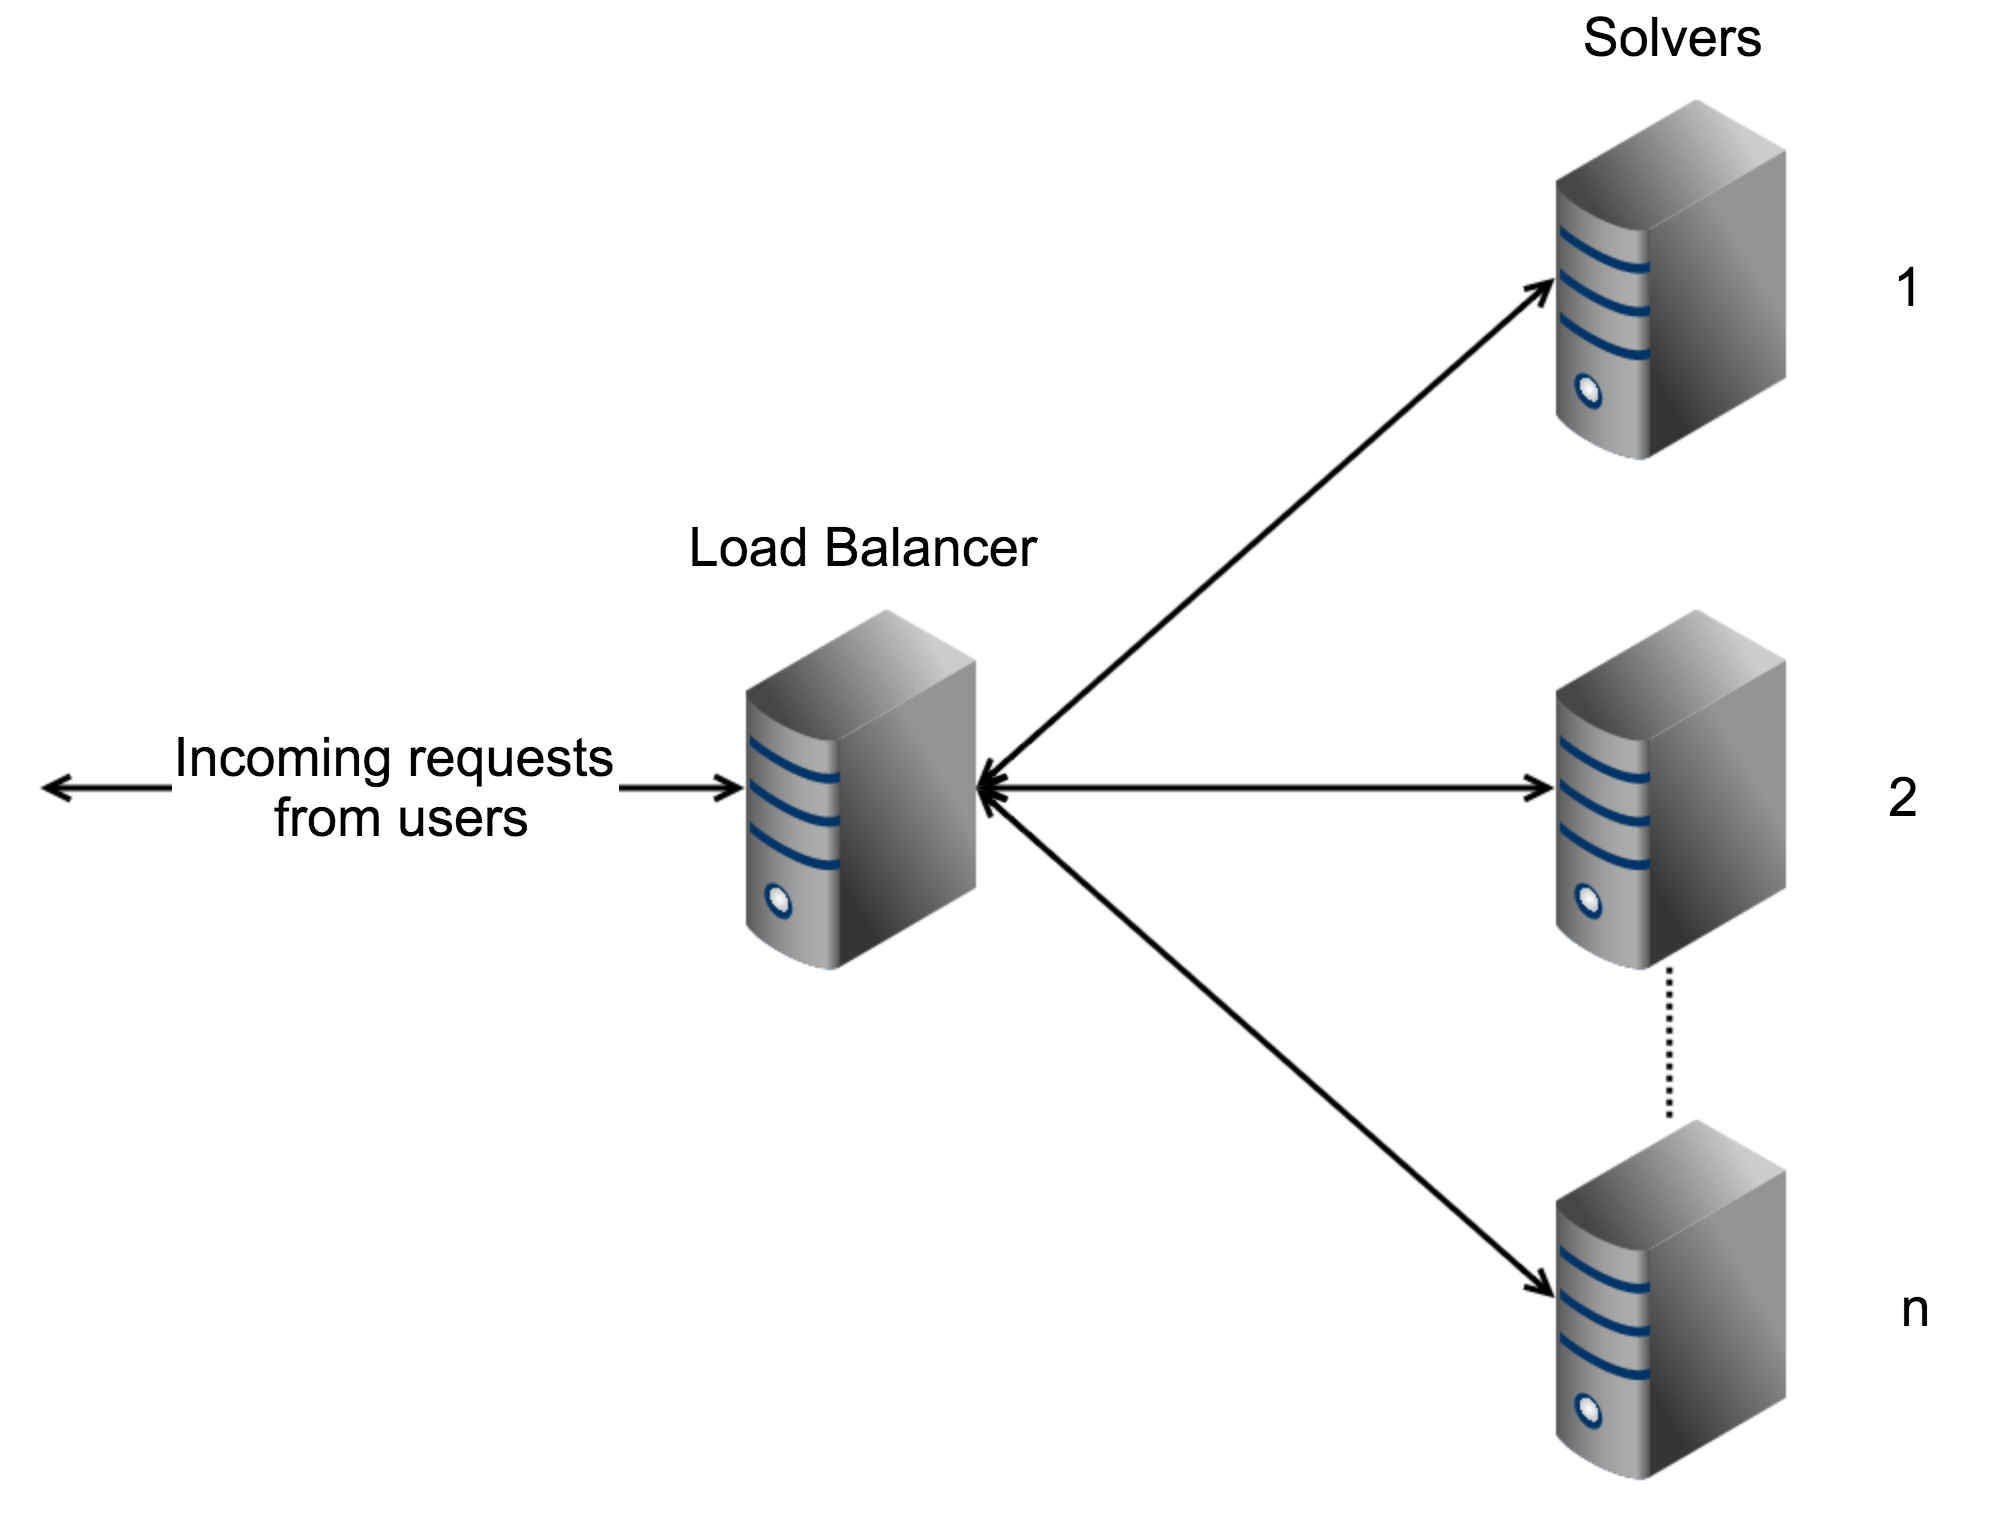
\includegraphics[width=0.5\textwidth]{img/arch}



%------------------------------------------------

\section{System Design}
System Design (recommended size: 1.5 pages)
\begin{enumerate}[(a)]
\item Resource Management Architecture: describe the design of your system,
including the inter-operation of the provisioning, allocation, reliability, and monitoring components (which correspond to the homonym features required by the WantCloud CTO).
\item System Policies: describe the policies your system uses and supports. The latter may remain not implemented throughout your coursework, as long as you can explain how they can be supported in the future.
\item (Optional) Additional System Features: describe each additional feature of your system, one sub-section per feature.
\end{enumerate}

%------------------------------------------------

\section{Experimental Results}
Experimental Results (recommended size: 1.5 pages)
\begin{enumerate}[(a)]
\item Experimental setup: describe the working environments (DAS, Amazon EC2,
etc.), the general workload and monitoring tools and libraries, other tools and libraries you have used to implement and deploy your system, other tools and libraries used to conduct your experiments.
\item Experiments: describe the experiments you have conducted to analyze each system feature, then analyze them; use one sub-section per experiment. For each experiment, describe the workload, present the operation of the system, and analyze the results. In the analysis, report:
\begin{enumerate}
\item Charged-time = time that would have been charged using the Amazon EC2 timing approach (1-hour increments)
\item Charged-cost = cost that would have been charged using the 3
E
Amazon EC2 charging approach, assuming 10 Euro-cents/charged hour
\item Service metrics of the experiment, such as runtime and response time of
the service, etc.
\item (optional) Usage metrics of the experiment, such as per-VM and overall
system usage and activity.
\end{enumerate}
\end{enumerate}

%------------------------------------------------

\section{Discussion}
Discussion (recommended size: 1 page): summarize the main findings of your work and discuss the tradeoffs inherent in the design of cloud-computing-based applications. Should the WantCloud CTO use IaaS-based clouds? Among others, use extrapolation of the results as reported in Section 6.b of the report, to discuss the charged time and the charged cost for 100,000/1,000,000/10,000,000 users and for 1 day/1 month/1 year.

%------------------------------------------------

\section{Conclusion}

%------------------------------------------------

\section{Appendix A: Time Sheets}

%----------------------------------------------------------------------------------------
%	REFERENCE LIST
%----------------------------------------------------------------------------------------

\begin{thebibliography}{99} % Bibliography - this is intentionally simple in this template

\bibitem{ec2}
Amazon EC2, http://aws.amazon.com/ec2/

\end{thebibliography}

%----------------------------------------------------------------------------------------

\end{multicols}

\end{document}
